\documentclass{beamer}
\usepackage{hyperref}
\usepackage{blindtext}
\usepackage{tikz}
\usepackage{media9}
\usepackage[utf8]{inputenc}
\graphicspath{{Media/}}
\usetheme{Execushares}

\title{Neuropsicología Introducción}
\subtitle{\large Clase 1}
\author{Pablo A. Reyes G.}
\date{Pontificia Universidad Javeriana}

\setcounter{showSlideNumbers}{1}

\begin{document}
	\setcounter{showProgressBar}{0}
	\setcounter{showSlideNumbers}{0}
	\frame{\titlepage}


	\begin{frame}
	\transfade
		\frametitle{Introducción}

				\begin{enumerate}
					\item Amalgama\\ \textcolor{ExecusharesGrey}{\hspace{1em}Biología, medicina, fisiología, matemáticas, filosofía, etc.}
					\pause
					\item Los de siempre - Los griegos, pero también estan los egipcios, los incas y hasta los chinos estudiaron el cerebro.
					\pause
					\item El impacto del estudio clínico-patológico entre 1861-1875  \\ \textcolor{ExecusharesGrey}{\hspace{1em}Descripciones de BROCA, Wernicke modelaron la primera neuropsicología --> Modelos neuronales del mecanismo subyacentes al lenguaje}
					\pause
					\item Fristh Hitzig 1870 \\ \textcolor{ExecusharesGrey}{\hspace{1em}Estimulación electrica \hspace{1em}Bases de la localización cerebral y la transmisión por vias eléctricas y no por los espírutis animales}
				\end{enumerate}	
	\end{frame}
	
	\setcounter{framenumber}{0}
	\setcounter{showProgressBar}{1}
	\setcounter{showSlideNumbers}{1}
		
\section{Historia}

		\begin{frame}
		\transfade
			\frametitle{Antiguedad y algo más}
			\begin{itemize}
				\item Aristóteles - Cerebro como órgano inútil vs el corazón.
				\pause
				\item Hipócrates (Grecia) - Cerebro/Pasiones-Mente?
				\pause
				\item Galeno (Roma) - Cerebro + Nervios (Espíritus animales)
				\pause
				\item Nemesius (Siria) - Teoría ventricular
				\pause
				\item Hipocrates y amigos Teoría de los Humores:bilis negra, bilis amarilla, flema y sangre
			\end{itemize}
		\end{frame}

\begin{frame}{Humores }
\transfade
\begin{figure}
    \centering
    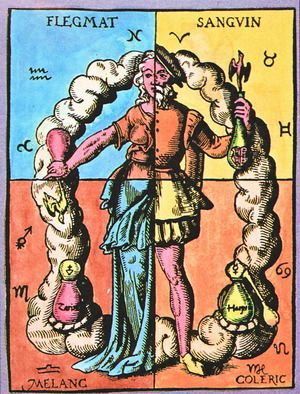
\includegraphics[height=0.75\paperheight]{humores.jpg}
    \caption{Temperamentos y características de personalidad / Salud Mental = desequilibrio}
    \label{fig:my_label}
\end{figure}
\centering
    
\end{frame}


\begin{frame}
	\transfade
	\frametitle{Renacimiento}
	\begin{figure}
\centering
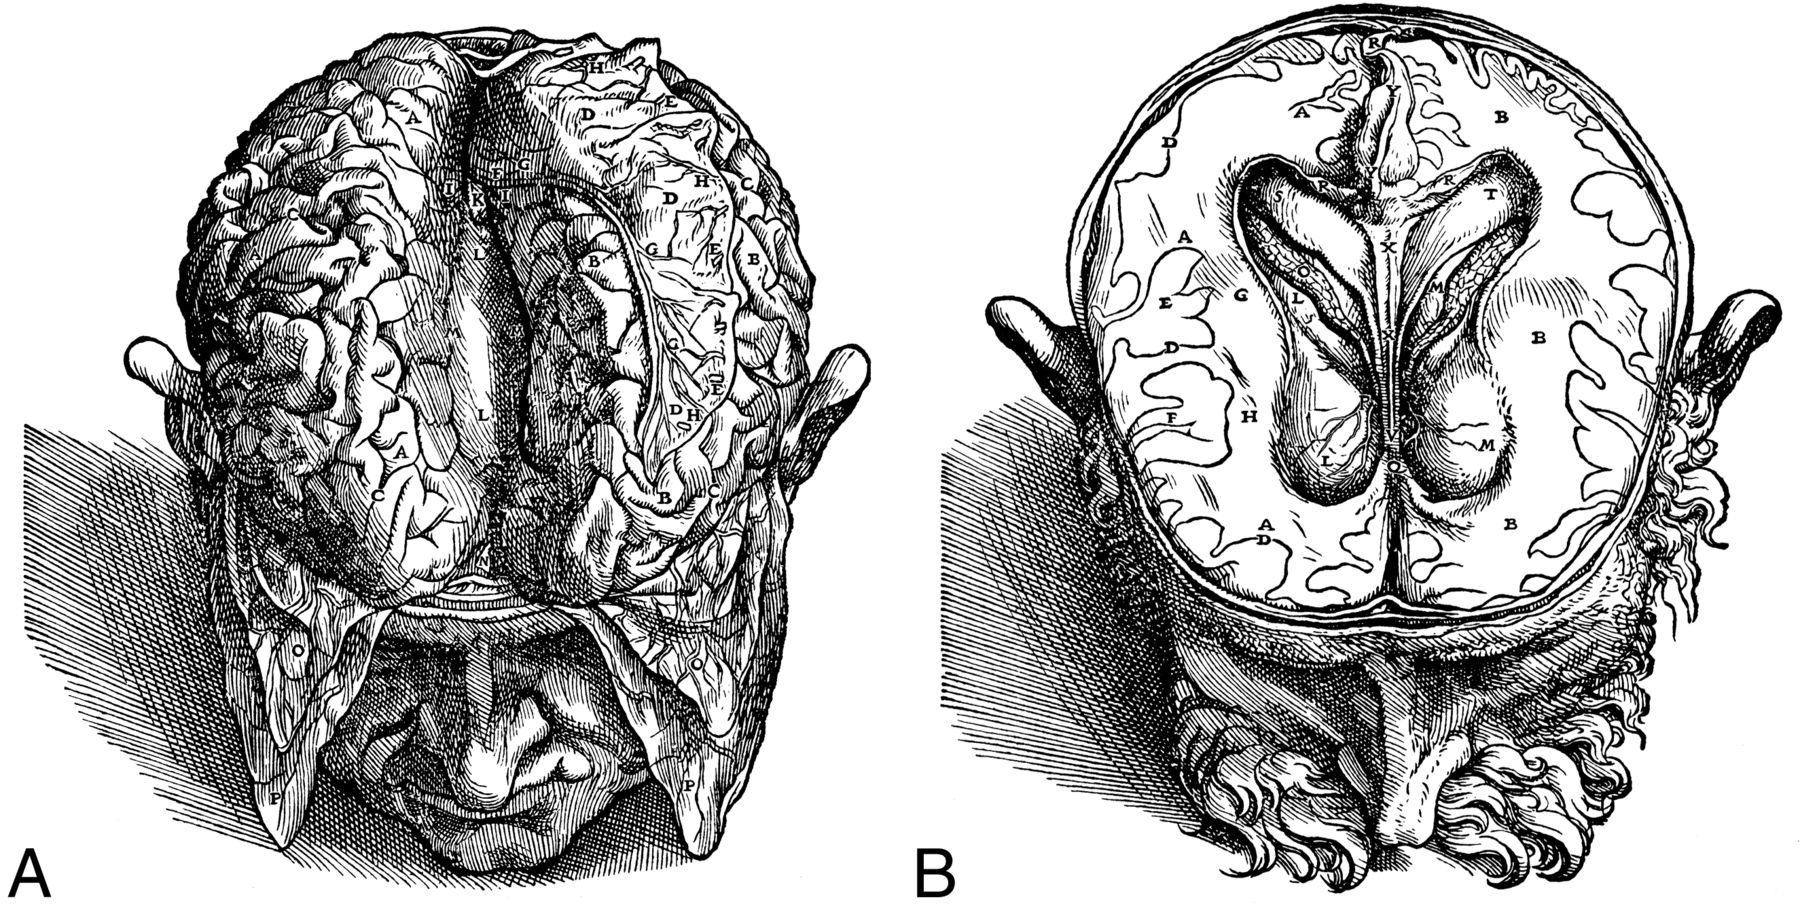
\includegraphics[width=1.1\linewidth]{vesalius1.jpg}
\caption{NVesalius como un padre para la neuroanatomia basada en disecciones}
\label{fig:ventriculos}
\end{figure}
\end{frame}

\begin{frame}{Cambio de paradigmas}
\transfade
\begin{columns}
\begin{column}{0.5\textwidth}
   \begin{itemize}
    \item Tal vez... los tiempos de dios no son perfectos.
    \pause
    \item El sol tiene manchas, la tierra no es el centro del universo. 
    \pause
    \item La anatomía antigua tiene errores.
\end{itemize}
\end{column}
\begin{column}{0.5\textwidth}  %%<--- here
    \begin{center}
     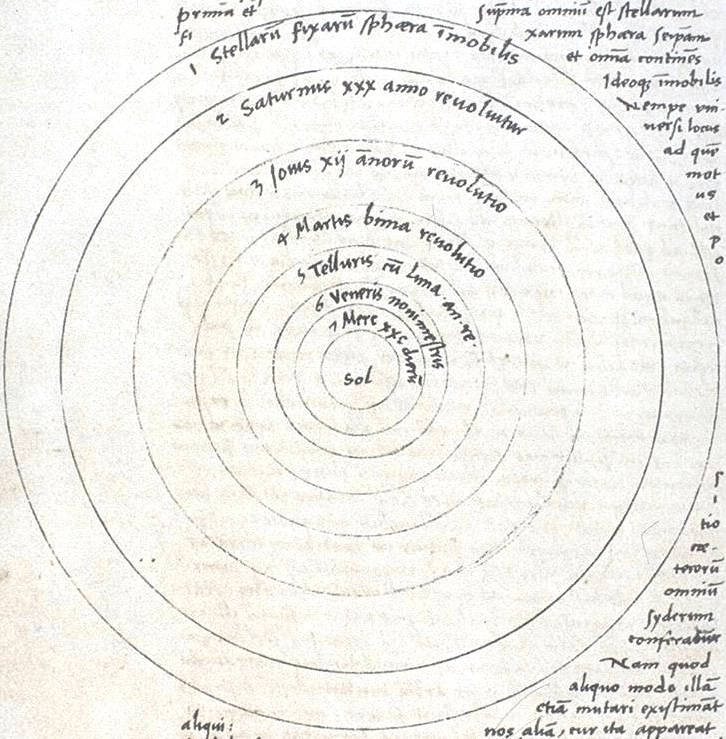
\includegraphics[width=1\textwidth]{heliocentrism.jpg}
     \end{center}
\end{column}
\end{columns}
\end{frame}

\section{Modernidad}

\begin{frame}{De la mecánica celeste a...}
\transfade
    \begin{columns}
    \begin{column}{0.5\textwidth}
        \begin{figure}
            \centering
            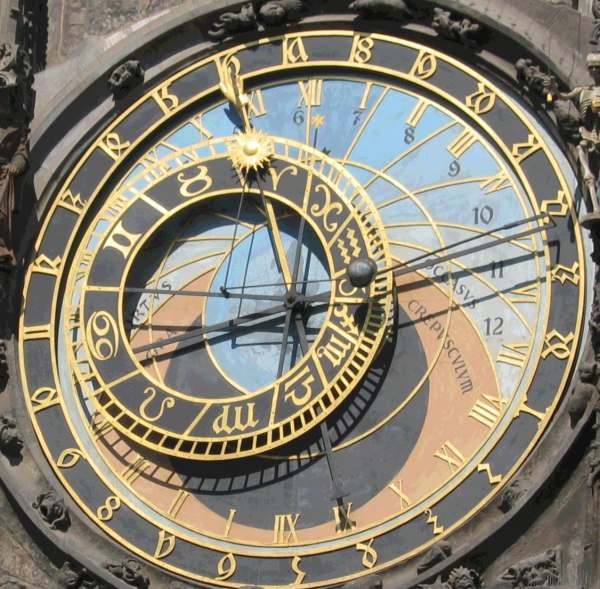
\includegraphics[width=1\linewidth]{reloj.jpg}
            \caption{Reloj de Praga 1462 - antes de américa}
            \label{fig:my_label}
        \end{figure}
    \end{column}
    \pause
    
    \begin{column}{0.5\textwidth}
        \begin{figure}
            \centering
            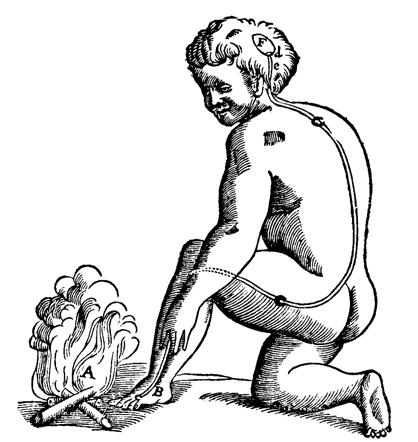
\includegraphics[width=1\linewidth]{descartes-reflejo.jpg}
            \caption{El reflejo, según descartes}
            \label{fig:my_label}
        \end{figure}
    \end{column}
    \end{columns}
\end{frame}

\begin{frame}{Pienso, luego...}
\transfade
    \begin{itemize}
        \item La duda por encima de todo... (menos de dios, claro).
        \pause
        \item El raciocinio como elemento central vs las pasiones.
        \pause
        \item Distinción entre animales y humanos, pero también similitudes por la forma de locomomoción.
        \pause
        \item leer Damasio.
    \end{itemize}
\end{frame}

\begin{frame}{Adiós espíritus animales}
\begin{figure}
    \centering
    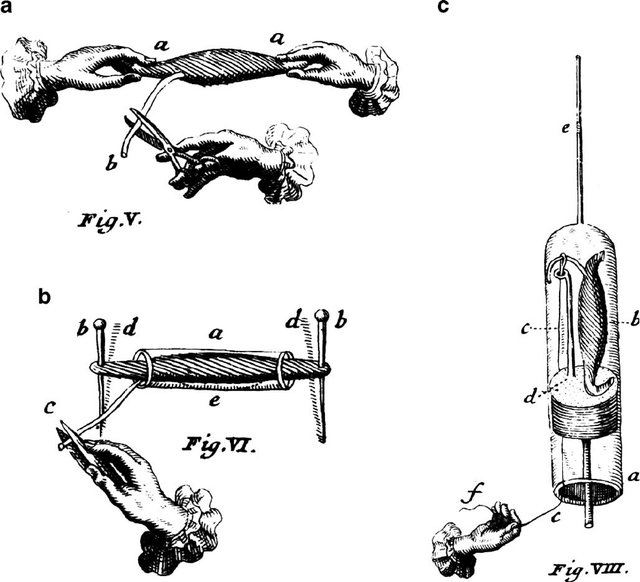
\includegraphics[width=0.65\linewidth]{musculossw.jpg}
    \caption{Experimento de Swammerdam 1758}
    \label{fig:my_label}
\end{figure}
\end{frame}

\begin{frame}{Electricidad animal}
    \transfade
    \begin{columns}
    \begin{column}{0.5\textwidth}
        \begin{figure}
            \centering
            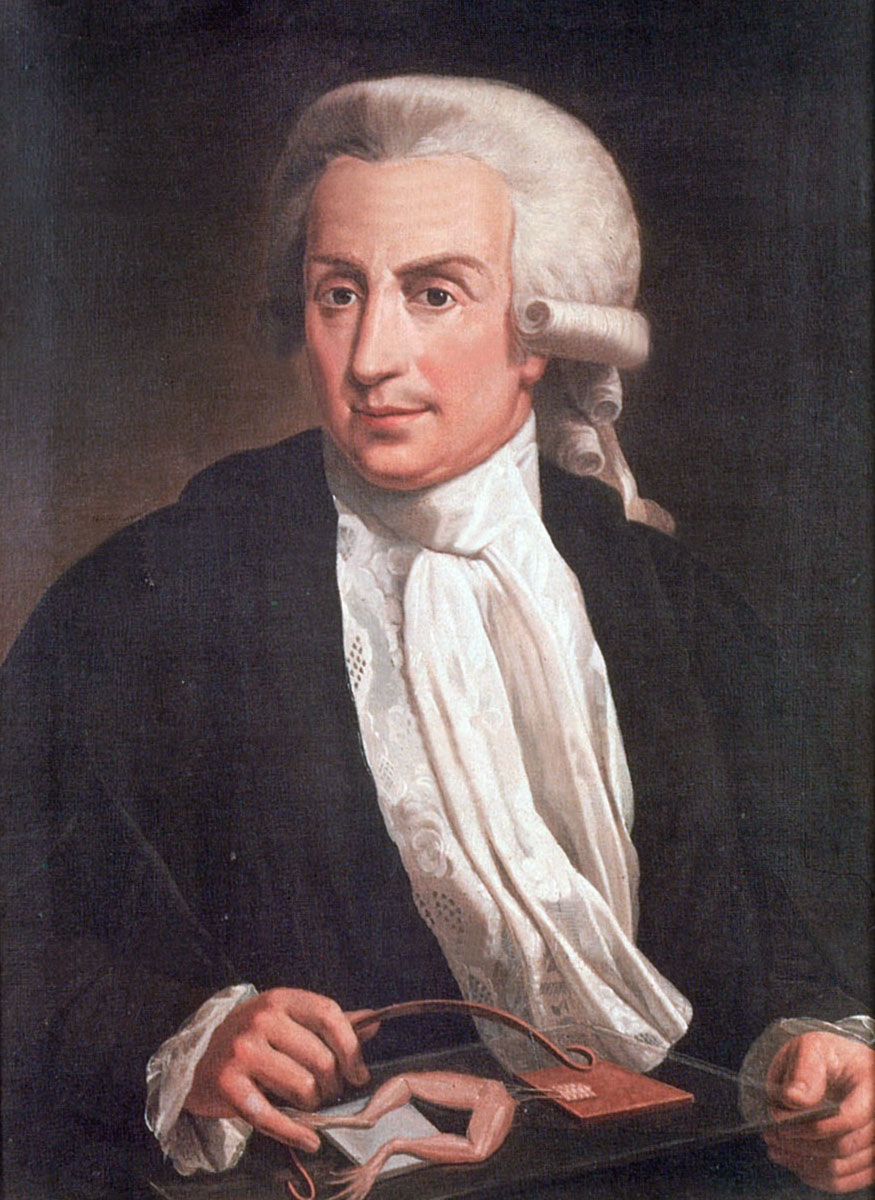
\includegraphics[width=0.9\linewidth]{galvani1.jpg}
            \caption{Galvani}
            \label{fig:my_label}
        \end{figure}
    \end{column}
    \pause
    
    \begin{column}{0.5\textwidth}
        \begin{figure}
            \centering
            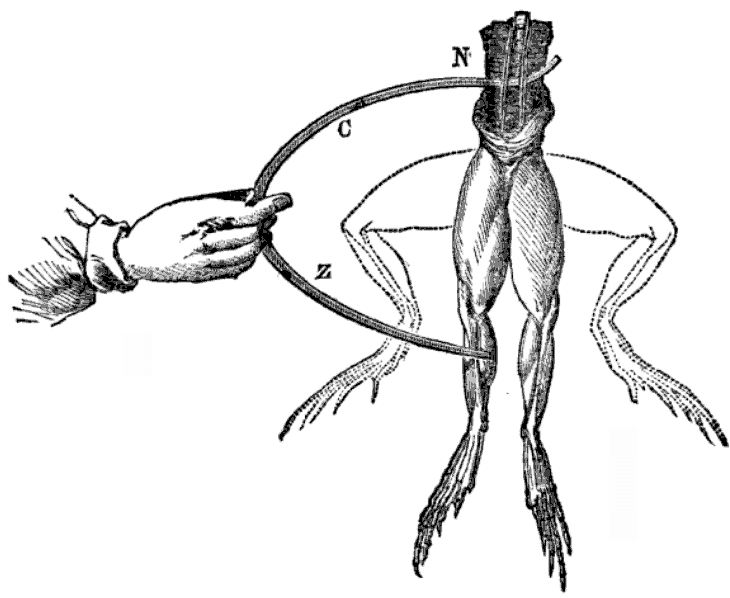
\includegraphics[width=1\linewidth]{galvani2.jpg}
            \caption{Corrientes Galvanicas}
            \label{fig:my_label}
        \end{figure}
    \end{column}
    \end{columns}
\end{frame}

\begin{frame}{Frenología}
	\transfade
\begin{columns}
\begin{column}{0.5\textwidth}
\begin{itemize}
    \item División en facultades mentales
    \item Cerebro / craneo / personalidad
    \item Es posible localizar las facultades mentales
    \item Joseph Gall
\end{itemize}
\end{column}
\pause
\begin{column}{0.5\textwidth}
\begin{figure}
    \centering
    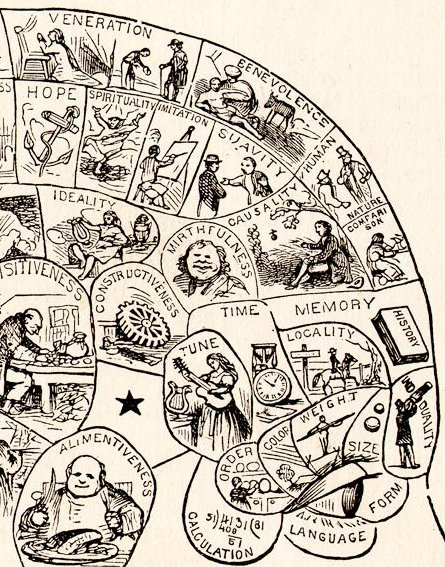
\includegraphics[width=0.9\linewidth]{frenologia1.jpg}
    \caption{Divisiones}
    \label{fig:my_label}
\end{figure}
\end{column}	
\end{columns}
\end{frame}

\begin{frame}{Sin embargo...}
    \transfade
    \begin{figure}
        \centering
        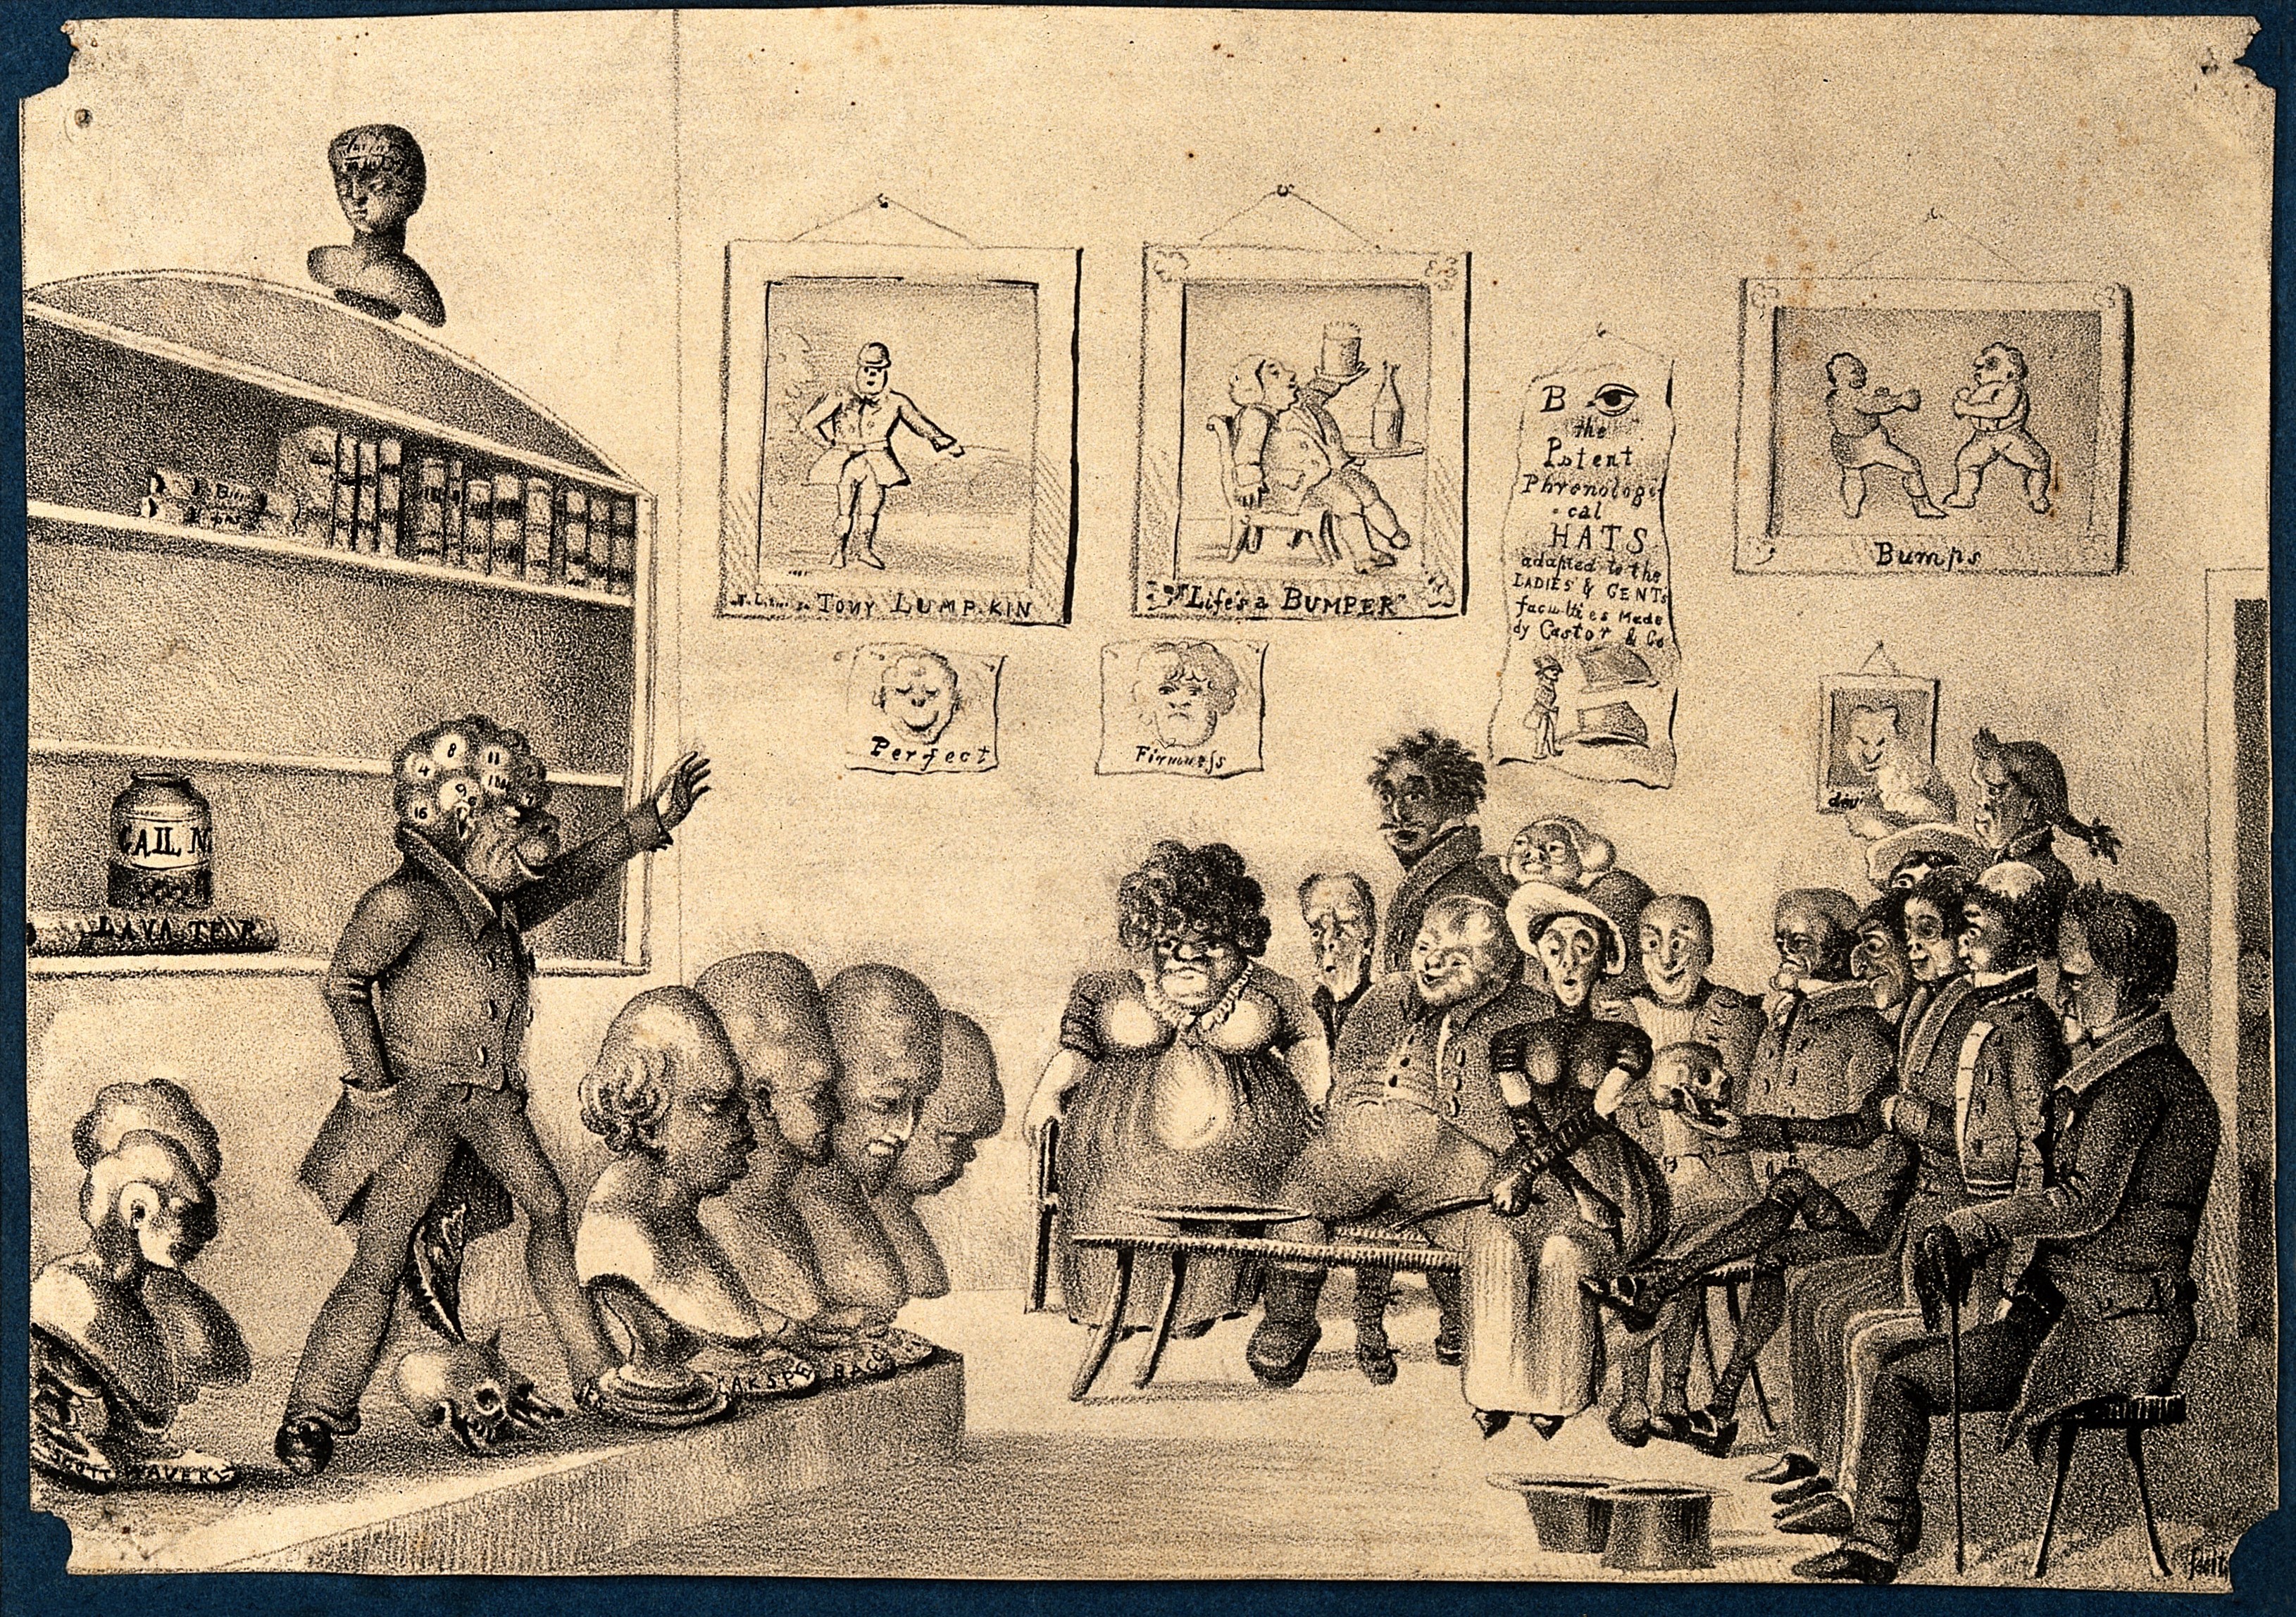
\includegraphics[width=0.9\linewidth]{caricaturafrenologia.jpg}
        \caption{Combe carizariturizado}
        \label{fig:my_label}
    \end{figure}
\end{frame}


		\begin{frame}
			\transfade
			\frametitle{Logros del localizacionismo}
			\begin{itemize}
				\item Ubicación de la corteza somatosensorial (giro precentral)
				\pause
				\item Visión (occipital)
				\pause
				\item Intelecto (Frontal)
				\pause
				\item Bases de la respiración y ritmos cardiacos (Tallo cerebral)
				\pause
				\item La Corteza contiene representaciones y las vías conectan diferentes representaciones.
				\pause
				\item Críticas... Jackson's (1878) "to locate the lesion which destroys speech and to locate speech are two different things"
				\pause
				\item Establecer que una lesión en X causa la pérdida de la funcion Y no es correcto.
				
			\end{itemize}
		\end{frame}

		\begin{frame}
			\transfade
			\frametitle{Otras posturas}
\begin{figure}
\centering
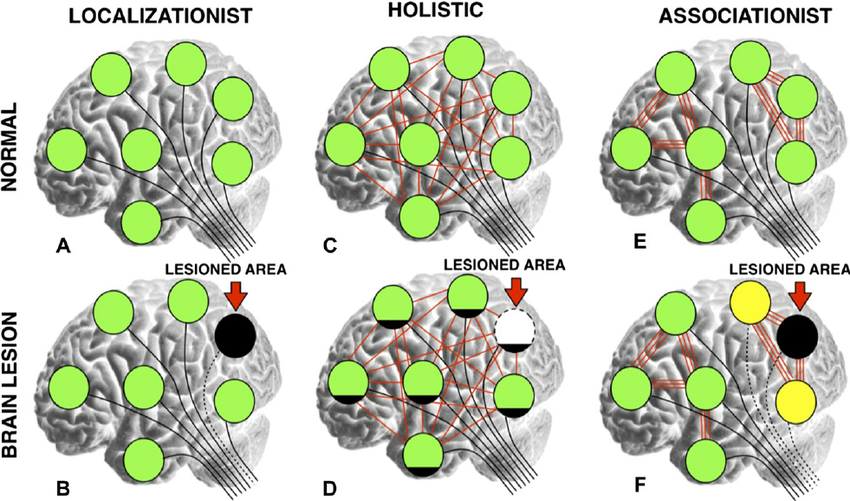
\includegraphics[width=1\linewidth]{localizacionistas.png}
\caption{Diferentes formas de entender la lesión}
\label{fig:localizacionistas}
\end{figure}
		\end{frame}

\section{Localización del lenguaje}

\begin{frame}{Los inicios}
\transfade
\begin{columns}
\begin{column}{0.5\textwidth}
\begin{figure}
    \centering
    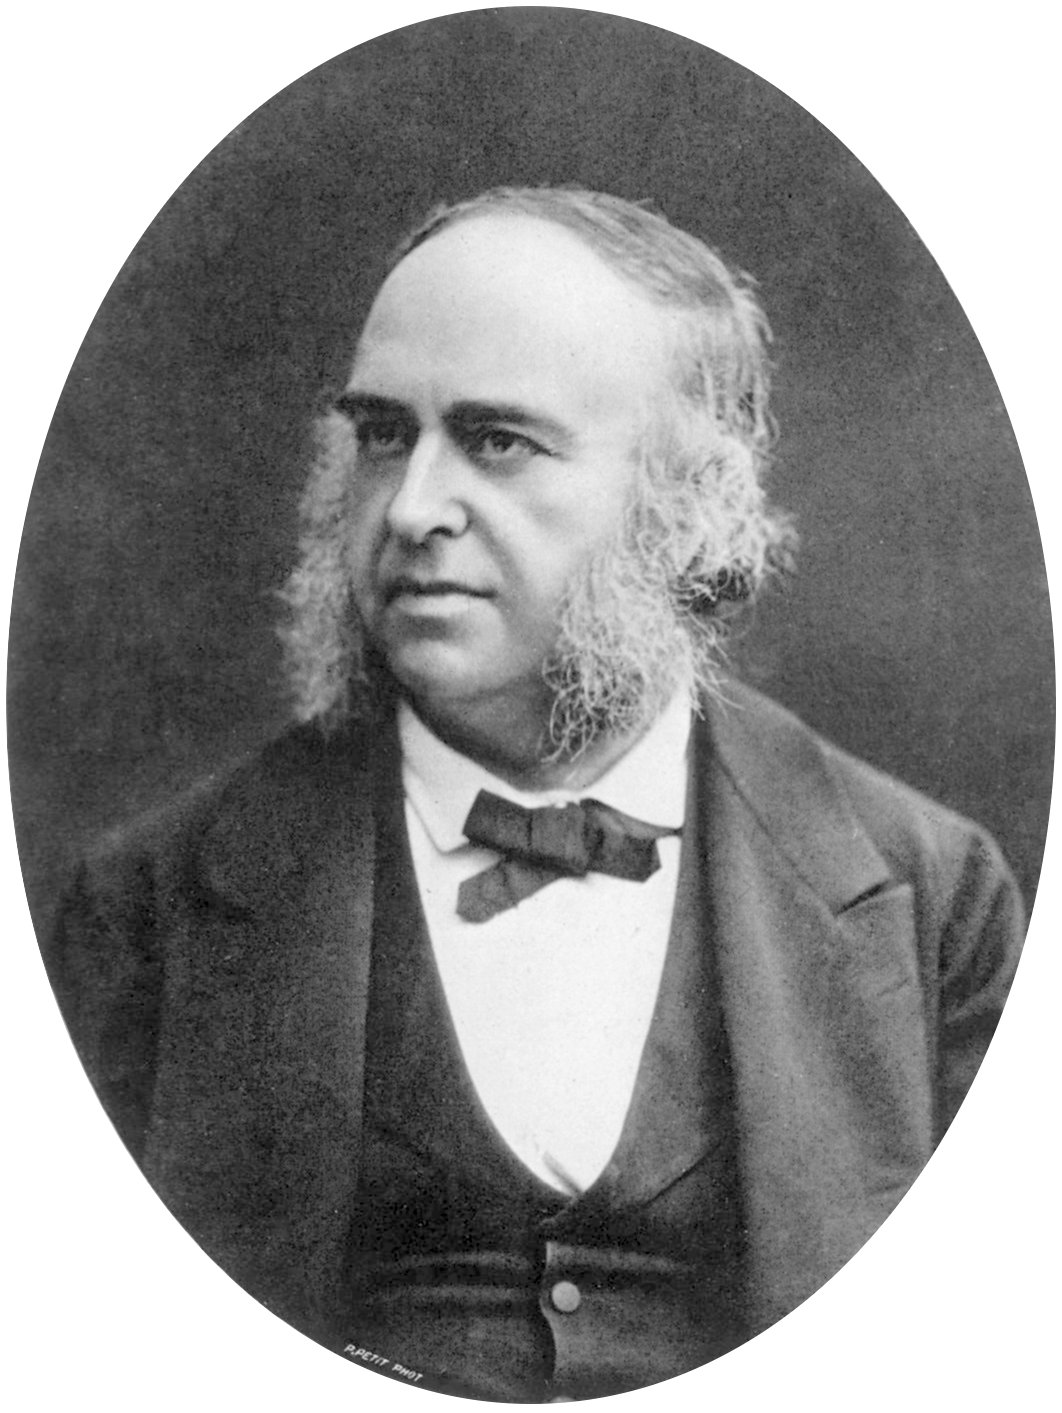
\includegraphics[width=0.8\linewidth]{Paul_Broca.jpg}
    \caption{Paul Broca / Tan / 1861 y 12 casos más}
\end{figure}
\end{column}
\begin{column}{0.5\textwidth}
\begin{figure}
    \centering
    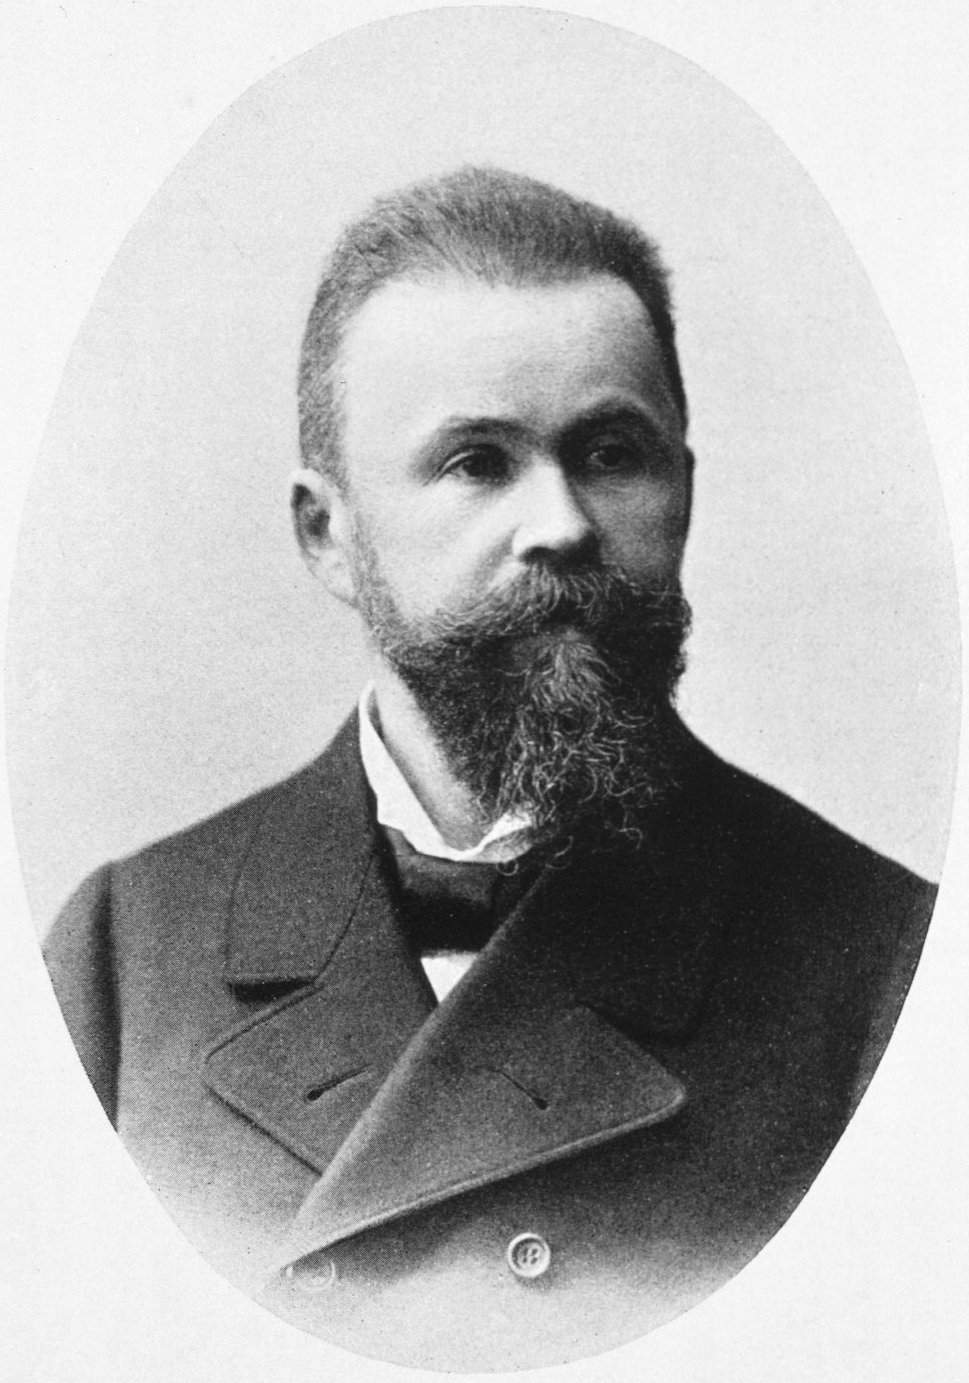
\includegraphics[width=0.8\linewidth]{Wernicke.jpg}
    \caption{Carl Wernicke / Mostró otros casos y otras regiones}
\end{figure}
\end{column}
\end{columns}
\end{frame}

\begin{frame}
\transfade
    \begin{figure}
        \centering
        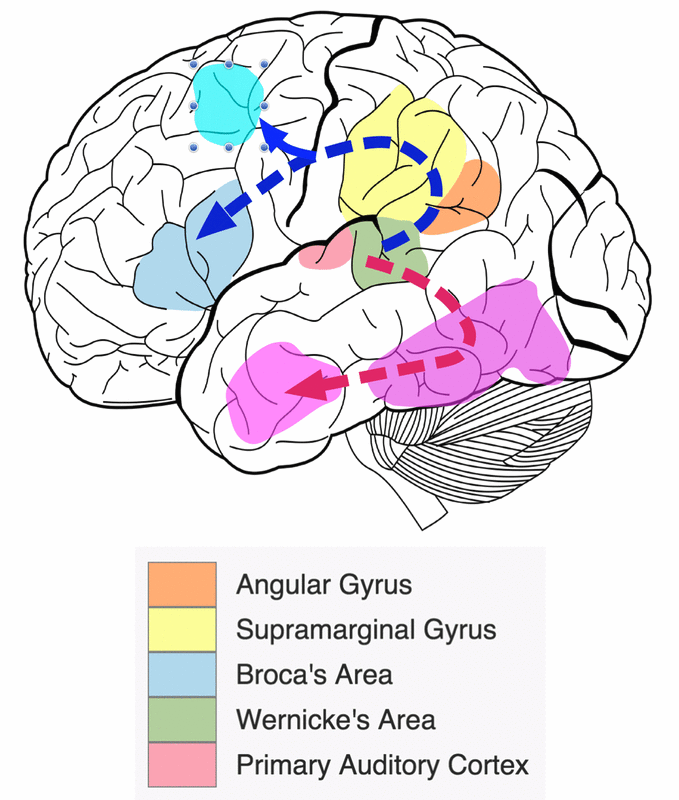
\includegraphics[width=0.7\linewidth]{broca1.png}
        
        \label{fig:my_label}
    \end{figure}
\end{frame}

\section{Hemisferios y dominancia}


\begin{frame}
    \begin{figure}
        \centering
        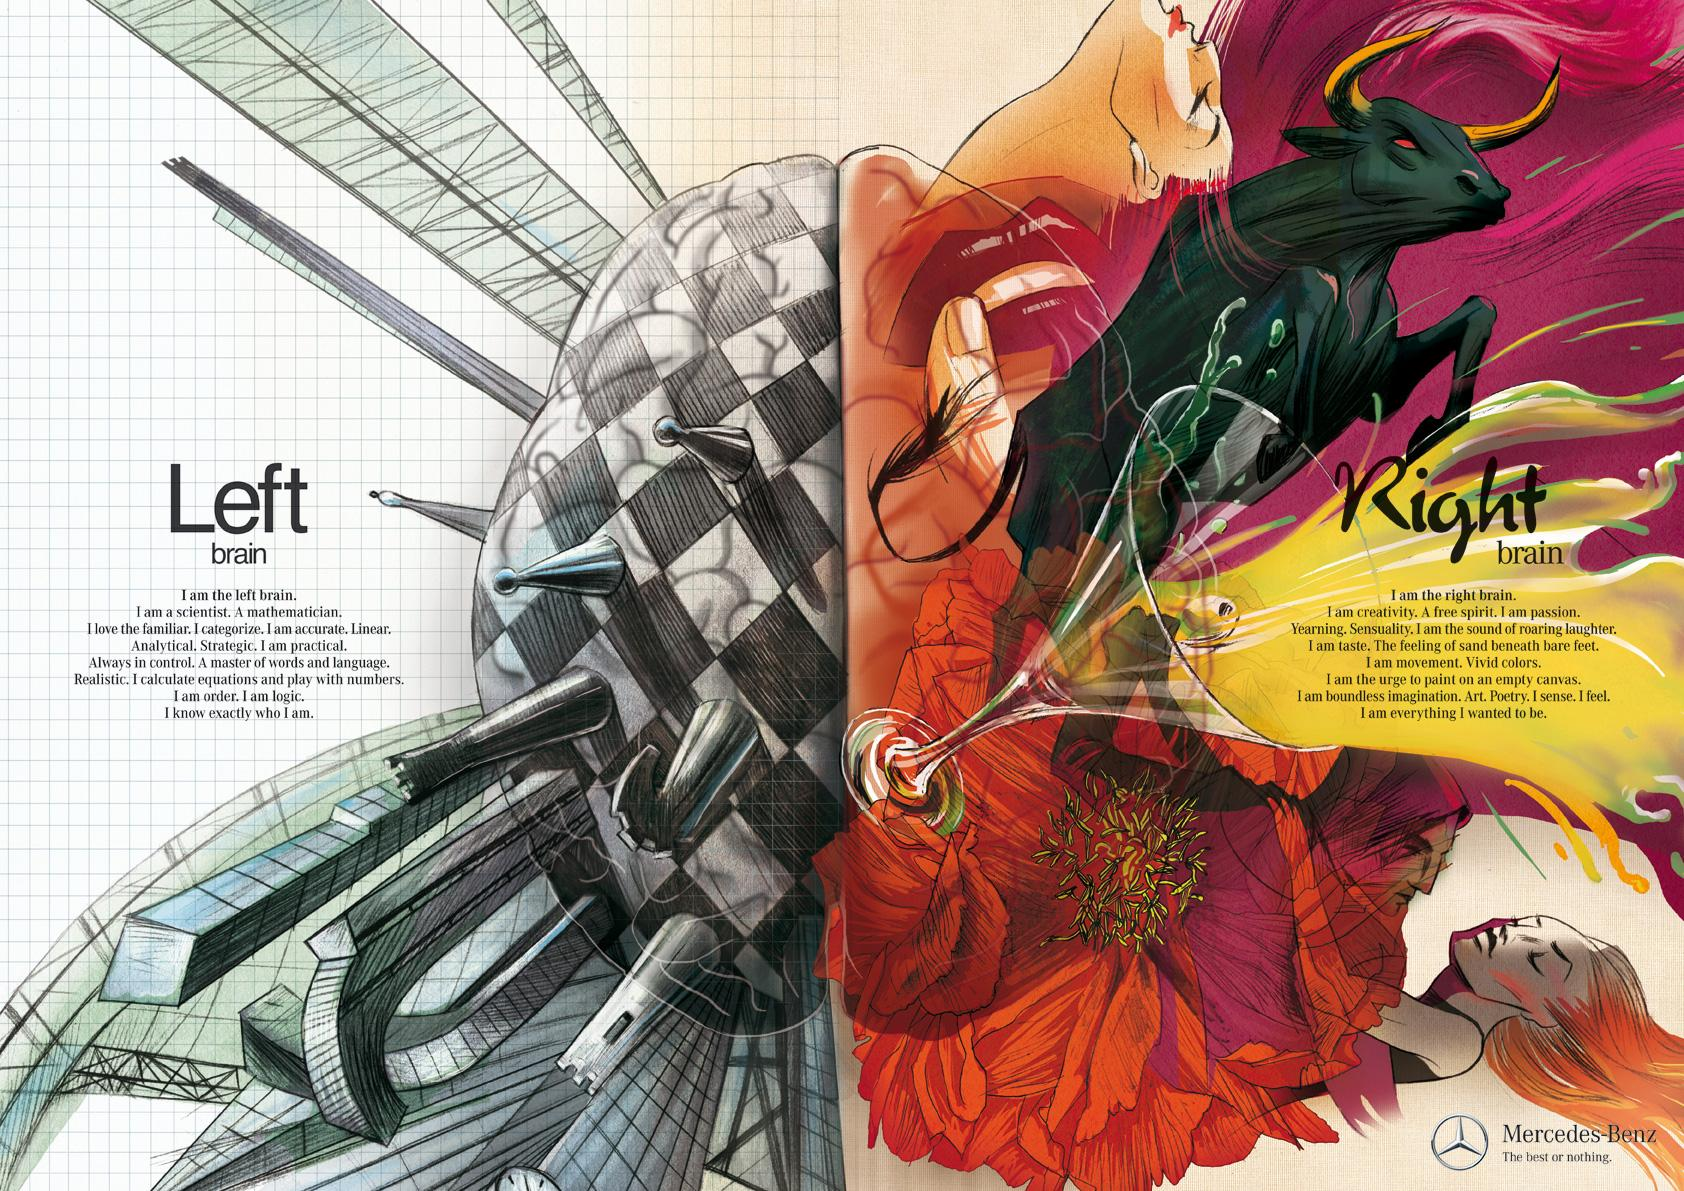
\includegraphics[width=1\linewidth]{izquierdo-derecho.jpg}
        %\caption{Caption}
        \label{fig:my_label}
    \end{figure}
\end{frame}


\begin{frame}
	\transfade
	\frametitle{derecho = ¿creatividad?}
	\begin{figure}
		\centering
		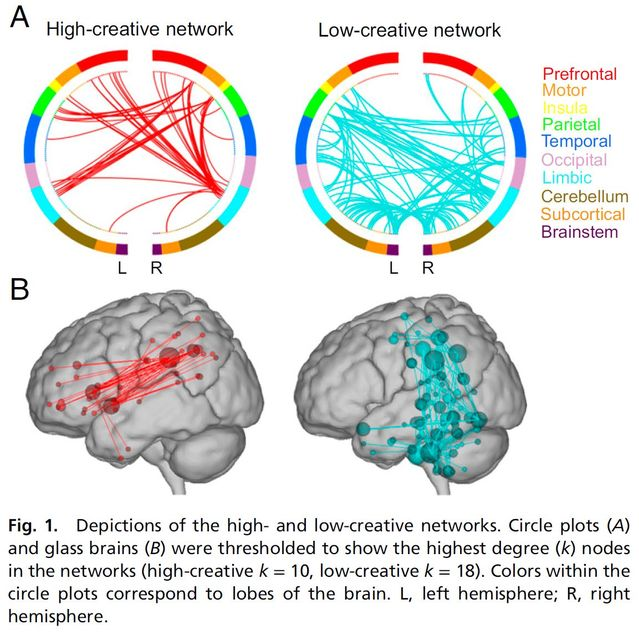
\includegraphics[width=0.7\linewidth]{brain_creativity_networks_2018.jpg}
		
		\label{fig:hemisferios}
	\end{figure}
	
\end{frame}


		\begin{frame}
			\transfade
			\frametitle{H. Izquierdo}
			\begin{itemize}
				\item Afasia en principio descrita como alteración del intelecto.
				\pause
				\item En el parietal: Esquema Corporal.
				\pause
				\item El hemisferio major vs el silente.
				\pause
				\item Diestros, con lesiones en HI en el frontal inferior producian AFASIA.
				\pause
				\item ZURDOS? en el HD produción AFASIA?
				\pause
				\item Conrad (1949) Demostraría que en zurdos ...
			\end{itemize}
		\end{frame}

\begin{frame}
	\transfade
	\frametitle{¿Dónde está el lenguaje?}
\centering
\includemedia[
  activate=pageopen,
  width=240pt,height=150pt,
  addresource=wada.mp4,
  flashvars={%
src=wada.mp4      % same path as in addresource!
%&scaleMode=stretch % removes black bars
&autoPlay=true      % optional configuration
&loop=true          % variables
}
]{}{StrobeMediaPlayback.swf}

\end{frame}


\begin{frame}
	\transfade
	\frametitle{¿Solamente Izquierdo?}
	\begin{itemize}
	\item Afasia
	\pause
	\item En el parietal: Esquema Corporal.
	\pause
	\item El hemisferio major vs el silente.
	\pause
	\item Diestros, con lesiones en HI en el frontal inferior producian AFASIA.
	\pause
	\item ZURDOS. ¿lesión en el HD produce AFASIA?
	\pause
	\item Conrad (1949) Demostraría que en zurdos ...
	\end{itemize}
\end{frame}

\begin{frame}
	\transfade
	\frametitle{¿Solamente Izquierdo? II}
	\begin{itemize}
		\item Remoción del H.I. el paciente puede producir lenguaje ligado a expresiones emocionales
	\end{itemize}
\end{frame}

\section{Lo no verbal}

\begin{frame}
	\transfade
	\frametitle{Más allá del H.D}
	\begin{itemize}
		\item Percepción visoespacial
		\pause
		\item Reactividad Emocional
		\pause
		\item Procesos atencionales
		\pause
		\item Otros
	\end{itemize}
\end{frame}
		

\end{document}
